\section{Park Details}
\label{parkDetails}

In den Details der einzelnen Parks gibt es eine \nameref{map} mit zwei Marker zu finden. Ein Marker für die 
Position des Parks und ein anderer für die derzeitige Position des Benutzers. Verweigert der 
Benutzer, dass auf seinen Standort zugegriffen werden darf, wird nur der Marker des Parks platziert.

\begin{figure}[H]
    \begin{center}
      \frame{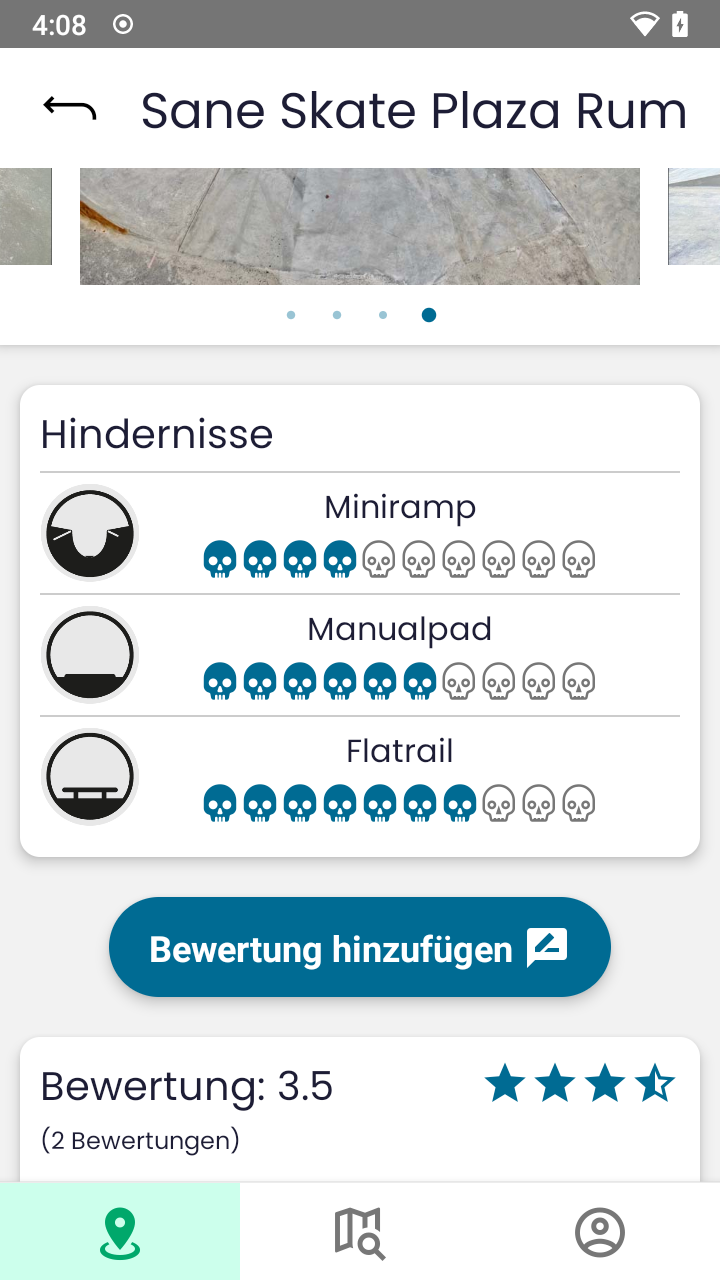
\includegraphics[width=1\textwidth]{Website/Obstacles.png}}
      \caption{Die Hindernisse}
    \end{center}
\end{figure}

Unterhalb der Map stehen die Hindernisse welche sich im Park befinden. Schwebt man mit der Maus 
über eins der Hindernisse wird der Name und die Schwierigkeit des Hindernisses angezeigt. Die Daten 
über das Hindernis und über den Park selbst, wird durch einen \textit{useFetch} in Erfahrung 
gebracht. Ist man mit einem Benutzer angemeldet, kann unter den Hindernissen eine Bewertung 
geschrieben werden.
\pagebreak
\subsection{Bewertungen}

\begin{figure}[H]
  \begin{center}
    \frame{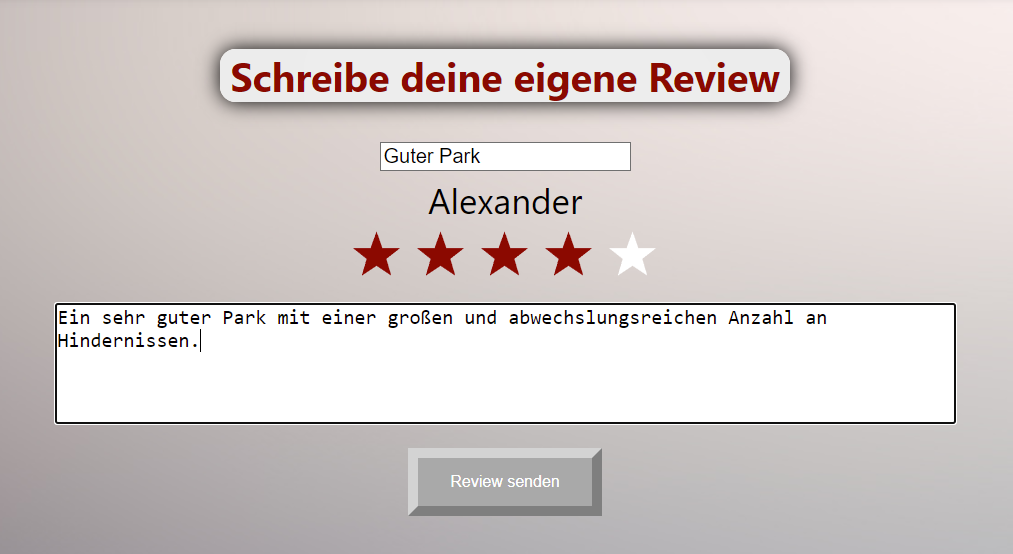
\includegraphics[width=1\textwidth]{Website/Review-Schreiben.png}}
    \caption{Eine Review schreiben}
  \end{center}
\end{figure}

Damit es möglich ist eine Review zu schreiben muss ein Titel angegeben werden. Unter dem Titel steht 
der Benutzername des eingeloggten Users. Mit einem Klick auf die Sterne kann wird dem Park eine 
Bewertung von eins bis fünf gegeben. Diese Sternenbewertung wurde mittels einer externen React 
Komponente names \textbf{React Star Ratings} von \textbf{ekeric13} gemacht. Drückt der Benutzer auf den 
Senden Knopf wird die Review an den Server gesendet.
Während die Review and den Server gesendet wird, ist der Knopf deaktiviert, damit bei wiederholten 
Knopfdruck nicht mehrere male eine Review and den Server gesendet wird.

\begin{figure}[H]
  \begin{center}
    \frame{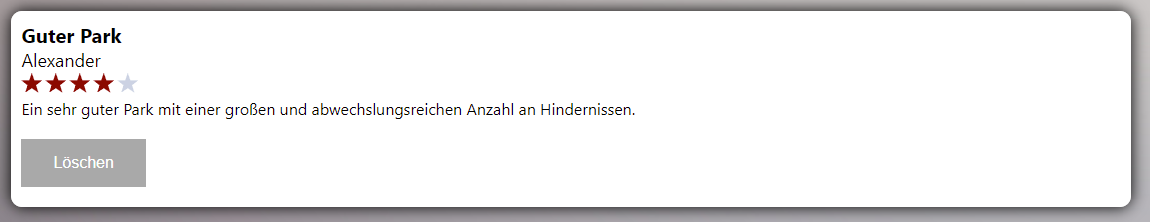
\includegraphics[width=1\textwidth]{Website/Review.png}}
    \caption{Eine geschriebene Bewertung}
  \end{center}
\end{figure}

Unter dem erstellen einer Bewertung befinden sich alle anderen Bewertungen dieses Park. Es ist möglich 
seine eigene Bewertung zu löschen. Dies erfolgt ganz einfach über die Überprüfung der BenutzerId
des eingeloggten Users, mit der BenutzerId des Herstellers der Bewertung.